\documentclass{beamer}
\usepackage{graphicx}
\usepackage{listings}
\graphicspath{ {./} }
\usepackage[utf8]{inputenc}


\title{While+ Interpreter}
\author{Visentin Filippo}

\begin{document}

\frame{\titlepage}

\begin{frame}
\frametitle{Task}
Design a While+ Interpreter I such that:
\begin{itemize}
	\item I takes as input any S $\in$ While+ and some representation of s $\in$ State
	\item I(S, s) must behave exactly as the $S_{ds}[S]s$ semantic tells
	\item I relies on Kleene-Knaster-Tarski fixpoint iteration sequence for evaluating the while statements
\end{itemize}
\end{frame}

\begin{frame}
	\frametitle{Interpreter structure}
	The interpreter is written in \textbf{Haskell}.
	It is composed of various modules:
	\begin{itemize}
		\item The \textbf{string parser}, to build the syntax tree
		\item The \textbf{syntax parser}, to match keywords and create statements
		\item The \textbf{interpreter}, to execute statements as stated by the $S_{ds}$
	\end{itemize}

\end{frame}
\begin{frame}
	\frametitle{String parser}
	Builds a syntax tree starting from the input program. \\
	It relies on parenthesis to distinguish \textbf{nested statements}
	\begin{figure}[h]
		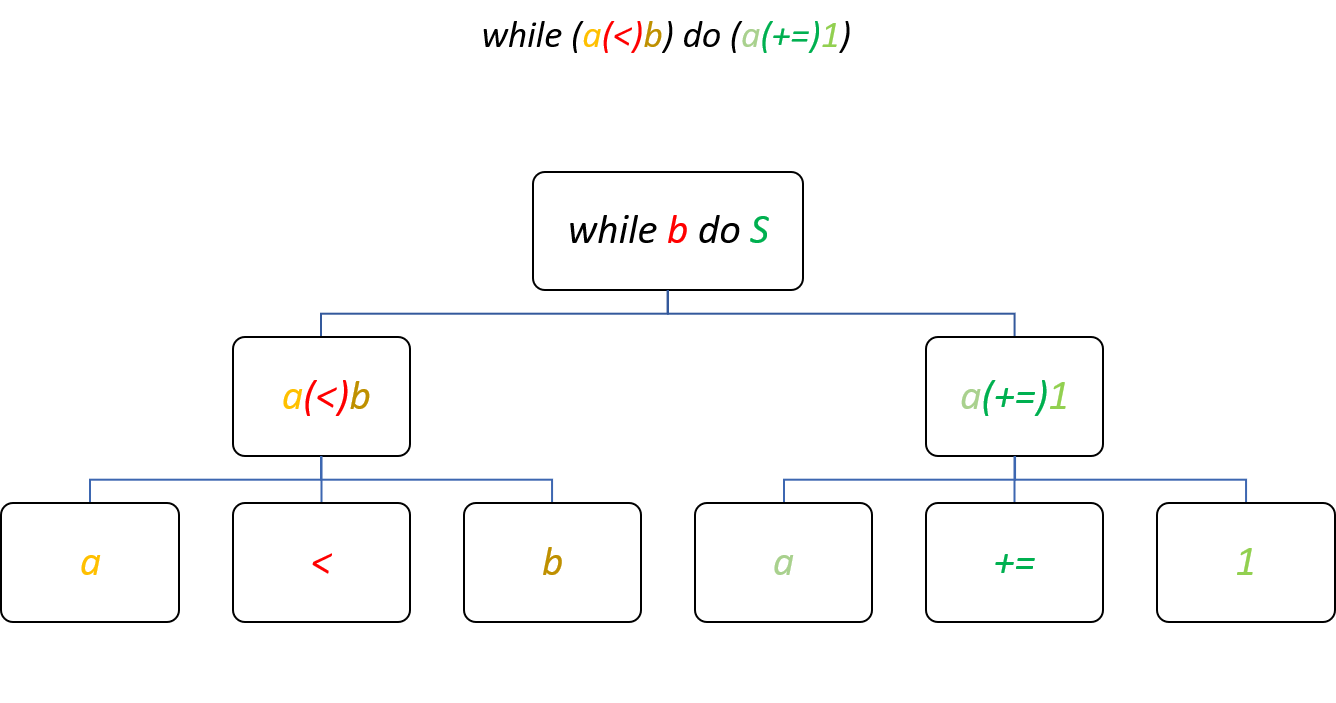
\includegraphics[width=8cm]{syntree}
	\end{figure}
\end{frame}

\begin{frame}
	\frametitle{Syntax parser}
	Starting from the syntax tree creates Haskell's types to encode the statements.\\
	It recursively traverses the tree composing types, each representing a different statement
	\begin{figure}[h]
		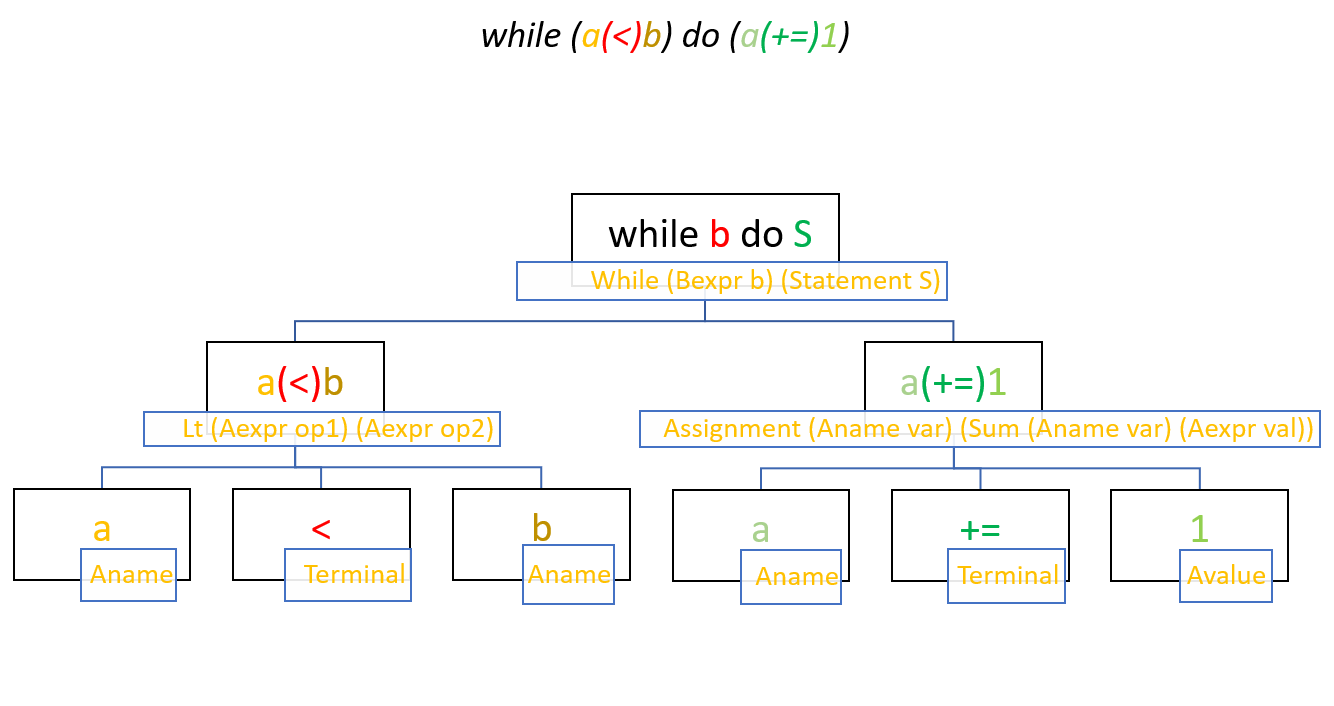
\includegraphics[width=8cm]{syntypes}
	\end{figure}
\end{frame}

\begin{frame}
	\frametitle{Interpreter}
	To give a semantics to the types I need to equip them with a function, distinguishing \textbf{expressions} (evalE) and \textbf{statements} (evalS). \\
	The 2 functions are overloaded, thanks to Haskell's pattern matching, to accomodate each expression variant.

\end{frame}

\begin{frame}
	\frametitle{While Statement}
	To implement the while semantics I started from the following observations: \\ \vspace{4mm}
	$\mathcal{D} : While \rightarrow \mathcal{P}(State) \hookrightarrow \mathcal{P}(State)$\\
	$\mathcal{D}$[while b do S]T = $B_c [\neg b](lfp(\lambda T'. T \cup (\mathcal{D}[s]\circ B_c[b]T')))$\\ \vspace{4mm}
	I start from a \textbf{precondition} and output a \textbf{postcondition} after the while. \\
	The precondition is a single state, so I get: \\ \vspace{4mm}
	$\mathcal{D} : While \rightarrow State \hookrightarrow \mathcal{P}(State)$\\ \vspace{4mm}
	
	I notice that the $lfp$ gives the invariant of the loop.
\end{frame} 
\begin{frame}
	\frametitle{While Statement}
	The Kleene-Knaster-Tarski fixpoint iteration is done to find this invariant. I need to apply this formulation until i get $FIX (F) = F$	\\ \vspace{4mm}
	Actually I observe that the only thing I need to keep of the invariant to get the exit state of the loop (if it terminates) is the \textbf{last state} computed by the procedure. \\ \vspace{4mm}
	$\mathcal{D} : While \rightarrow State \hookrightarrow State$\\ \vspace{4mm}
	So I can modify the procedure discarding other elements, not performing the union:\\ \vspace{4mm} 
	$lfp(\lambda T'. \mathcal{D}[s]\circ B_c[b]T')$ \\ \vspace{4mm}
	Also care must be taken if the loop does not \textbf{terminate}. If the fixpoint terminates, giving an invariant but the guard is still true, the wanted behaviour is to keep going with the iteration forever.
\end{frame}
\end{document}